\section{评估}
\label{kvdirect:sec:eval}

\begin{figure}[t]
\subfloat[固定内存利用率 0.5。\label{kvdirect:fig:optimize_fix_mem}]
{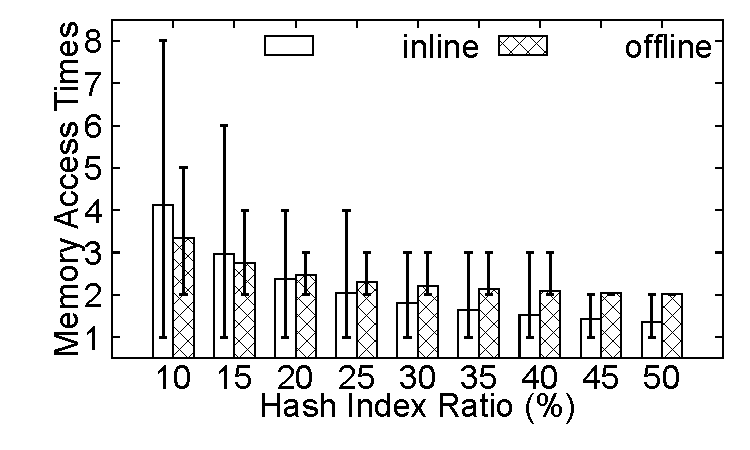
\includegraphics[width=.5\textwidth,page=1]{fix_mem.pdf}}
\subfloat[固定哈希索引率 0.5。\label{kvdirect:fig:optimize_fix_ratio}]
{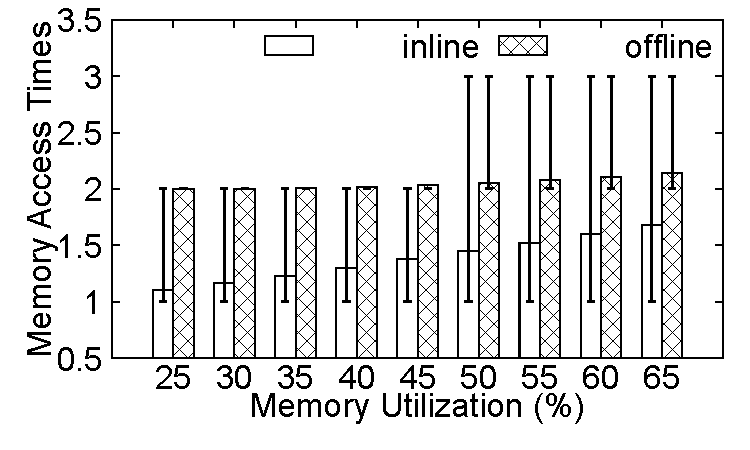
\includegraphics[width=.5\textwidth,page=1]{fix_ratio.pdf}}
\caption{不同内存利用率或哈希索引率下的内存占用。}
\label{kvdirect:fig:memory-access-count}
\end{figure}

\label{kvdirect:sec:evaluation}
在本节中,我们首先采用简化视角来支持我们的设计选择,使用关键组件的微基准,然后切换到整体方法,以演示系统基准中\oursys {}的整体性能。


我们在8台服务器和1台Arista DCS-7060CX-32S交换机的测试台上评估键值-Direct。
每台服务器配备两个禁用超线程的8核Xeon E5-2650 v2 CPU,形成两个通过QPI Link连接的NUMA节点。每个NUMA节点都装有8个DIMM 8~GiB三星DDR3-1333 ECC RAM,每台服务器上总共有128~GiB的主机内存。
可编程NIC~ \cite {caulfield2016cloud}连接到CPU 0的PCIe根联合体,其40~Gbps以太网端口连接到交换机。可编程NIC在分叉的Gen3 x16物理连接器中有两个PCIe Gen3 x8链路。
经过测试的服务器配备SuperMicro X9DRG-QF主板和一个运行Archlinux的120~GB SATA SSD(内核版本4.11.9-1)。

对于系统基准测试,我们使用YCSB工作负载 \cite {cooper2010benchmarking}。
对于偏斜(skewed)的Zipf工作负载,我们选择偏差(skewness)0.99并将其称为\textit {长尾}工作负载。

\subsection{微基准测试}
\label{kvdirect:sec:microbenchmarks}


\begin{figure}[t]
\centering
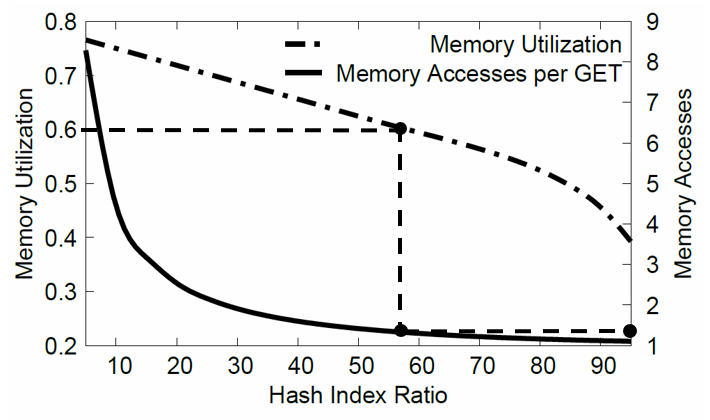
\includegraphics[width=0.6\textwidth,page=1]{optimize.png}
\caption{如何在给定内存利用率需求和 键值 大小的情况下决定最优哈希索引率。}
\label{kvdirect:fig:hashline-ratio}

\end{figure}

\subsubsection{哈希表}
\label{kvdirect:sec:hashtable-eval}

我们的哈希表设计中有两个自由参数:(1)内联阈值,(2)整个内存空间中哈希索引的比率。
如图\ref {kvdirect:fig:optimize_fix_mem}所示,当哈希索引比率增长时,可以内联存储更多的键值对,从而产生更低的平均内存访问时间。
图\ref {kvdirect:fig:optimize_fix_ratio}显示了随着使用更多内存而增加的内存访问量。
如图\ref {kvdirect:fig:hashline-ratio}所示,最大可实现内存利用率在较高哈希索引比率下下降,因为可用于动态分配的内存较少。
因此,为了在给定的存储器大小中容纳整个语料库,哈希索引比率具有上限。
我们选择此上限并获得最小的平均内存访问时间,如图\ref {kvdirect:fig:hashline-ratio}中的虚线所示。

\begin{figure}[t]
\centering
\subfloat[10B GET.\label{kvdirect:fig:mem-access-10-get}]
{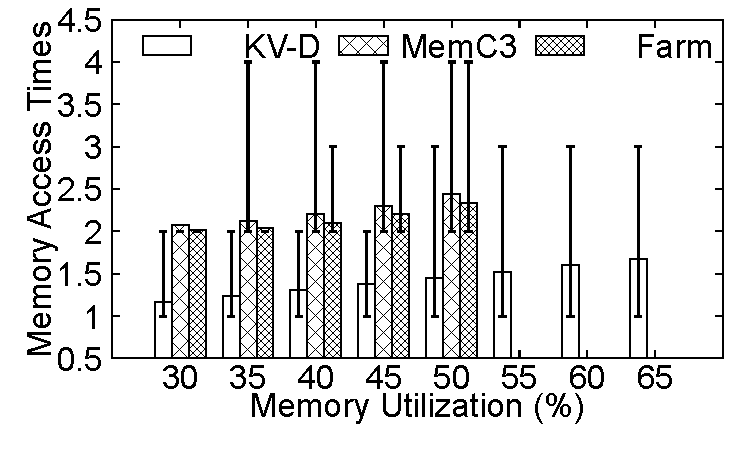
\includegraphics[width=.5\textwidth,page=1]{10B_get.pdf}}
\subfloat[10B PUT.\label{kvdirect:fig:mem-access-10-put}]
{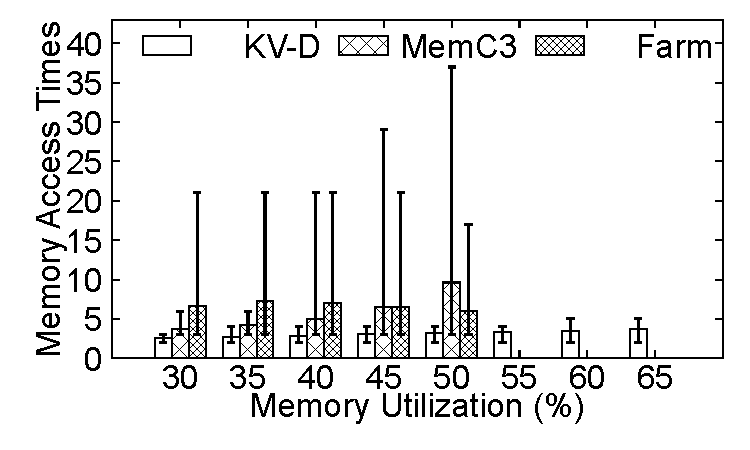
\includegraphics[width=.5\textwidth,page=1]{10B_put.pdf}}

\vfill

\subfloat[254B GET.\label{kvdirect:fig:mem-access-254-get}]
{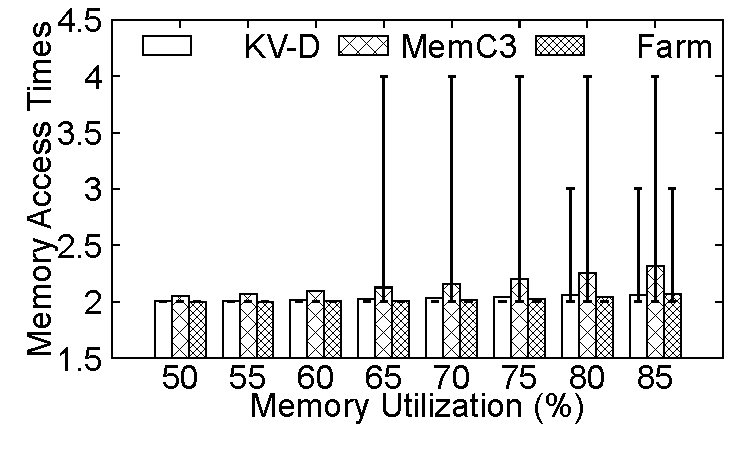
\includegraphics[width=.5\textwidth,page=1]{254B_get.pdf}}
\subfloat[254B PUT.\label{kvdirect:fig:mem-access-254-put}]
{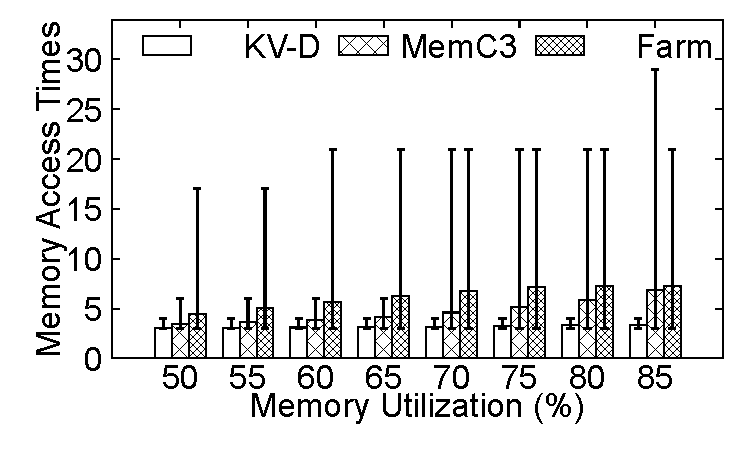
\includegraphics[width=.5\textwidth,page=1]{254B_put.pdf}}
\caption{每个 键值 操作的内存访问次数。}
\label{kvdirect:fig:mem-access-tput}

\end{figure}

在图\ref {kvdirect:fig:mem-access-tput}中,我们绘制了三种可能的哈希表设计的每个GET和PUT操作的内存访问次数:在键值-Direct中链接,MemC3中的桶式布谷鸟哈希(bucketized Cuckoo Hash)\cite {fan2013memc3}和FaRM \cite {dragojevic2014farm}中的链式关联(chain associative)跳房子散列(Hopscotch Hash)。
对于键值-Direct,我们针对给定的键值大小和内存利用率要求,为内联阈值和哈希索引比率做出最佳选择。
对于布谷鸟和跳房子散列,我们假设键是内联的并且可以并行比较,而值存储在动态分配的板中。
由于MemC3和FaRM的哈希表不能支持10B 键值大小超过55%的内存利用率,图\ref {kvdirect:fig:mem-access-10-get}和图\ref {kvdirect:fig:mem-access-10-put}仅显示键值-Direct的性能。

对于内联键值,键值-Direct在每个GET上接近1个内存访问,在非极端内存利用率下每个PUT接近2个内存访问。
非内联键值的GET和PUT有一个额外的内存访问。
在高内存利用率下比较键值-Direct和链式跳房子散列,跳房子散列在GET中表现更好,但在PUT中表现更差。
虽然键值-Direct无法保证最坏情况下的DMA访问,但我们会在GET和PUT之间取得平衡。
布谷鸟散列需要在GET上访问最多两个散列槽,因此在大多数内存利用率下,键值-Direct具有更多的内存访问。
在高内存利用率下,布谷鸟散列会导致每个PUT的内存访问时间出现大幅波动。


\begin{figure}[t]
\centering
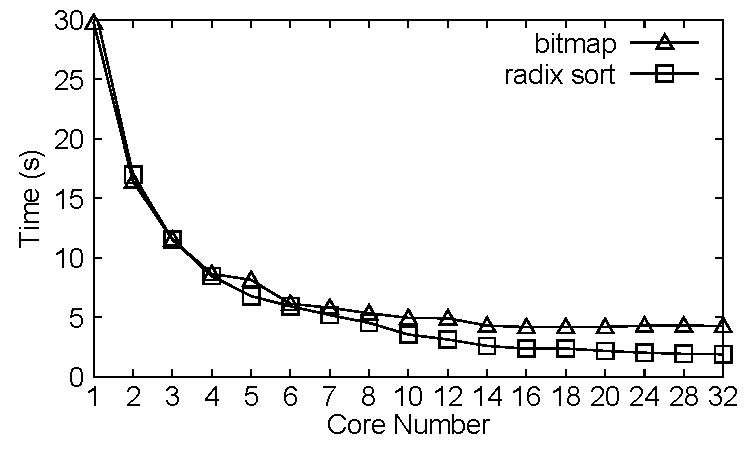
\includegraphics[width=0.6\textwidth]{slab-gc.pdf}
\caption{合并 40 亿个 slab 槽位的时间开销。}
\label{kvdirect:fig:slab-garbage-collection}

\end{figure}

\subsubsection{Slab 内存分配器}
\label{kvdirect:sec:slab-eval}

slab内存分配器的通信开销来自NIC访问主机内存中的可用slab队列。
为了维持每秒180M操作的最大吞吐量,在最坏的情况下,需要传输180M平板插槽,消耗720 MB / s PCIe吞吐量,即我们NIC的总PCIe吞吐量的5%。

slab内存分配器的计算开销来自主机CPU上的slab拆分和合并。
幸运的是,它们并不经常被调用。
对于具有稳定键值大小分布的工作负载,新释放的slab槽由后续分配重用,因此不会触发拆分和合并。

板坯分裂需要将连续的板坯条目从一个板坯队列移动到另一个板坯队列。当工作负载从大键值转换到小键值时,在最坏的情况下,CPU需要每秒移动90M板条目,这只占核心的10%,因为它只是连续的内存复制。

将自由平板槽合并到较大的槽是相当耗时的任务,因为它涉及用可能随机的偏移填充分配位图,因此需要随机存储器访问。
要对自由平板的地址进行排序并合并连续的平板,基数排序 \cite {satish2010fast} 可以比简单的位图更好地扩展到多个内核。
如图\ref {kvdirect:fig:slab-garbage-collection} 所示,将16 GiB向量中的所有40亿个空闲 slab 槽位合并在一个内核上需要30秒,或者在32个内核上使用基数排序仅需1.8秒 \cite{satish2010fast}。
虽然垃圾收集空闲 slab 槽位需要几秒钟,但它在后台运行而不会停止 slab 分配器,并且实际上仅在工作负载从小键值转换到大键值时触发。

\begin{figure}[t]
\centering
\subfloat[原子操作。\label{kvdirect:fig:ooo-atomic}]
{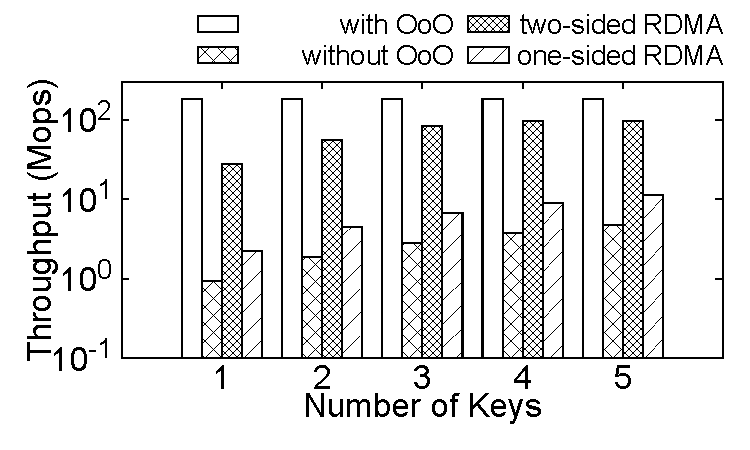
\includegraphics[width=.5\textwidth,page=1]{ooo_atomic.pdf}}
\subfloat[长尾负载。\label{kvdirect:fig:ooo-longtail}]
{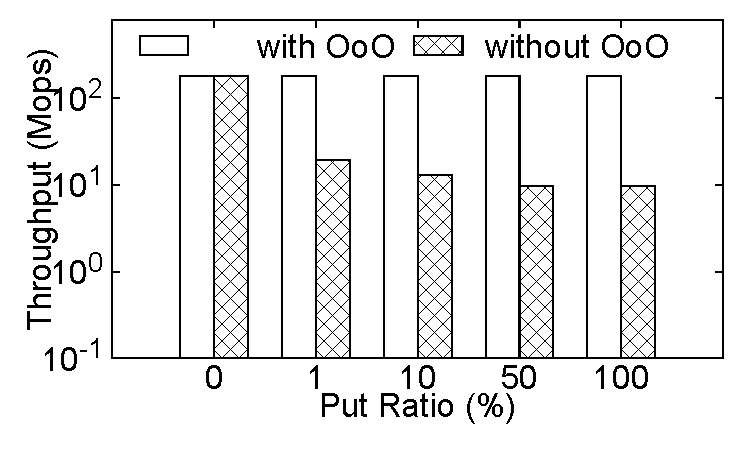
\includegraphics[width=.5\textwidth,page=1]{ooo_long-tail.pdf}}
\caption{乱序执行引擎的效率。}
\label{kvdirect:fig:ooo-eval}

\end{figure}


\subsubsection{乱序执行引擎}
\label{kvdirect:sec:ooo-eval}

我们通过比较吞吐量和在原子和长尾工作负载下使关键冲突管道停滞的简单方法来评估乱序执行的有效性。单面RDMA和双面RDMA \cite {kalia2016design}吞吐量也显示为基线。

如果没有此引擎,原子操作需要等待NIC中的PCIe延迟和处理延迟,在此期间无法执行对同一密钥的后续原子操作。
这使得单键原子吞吐量在图 \ref{kvdirect:fig:ooo-atomic} 中为0.94~Mops,与从RDMA NIC测量的2.24~Mops一致 \cite {kalia2016design}。
RDMA NIC的更高吞吐量可归因于其更高的时钟频率和更低的处理延迟。
对于无序执行,键值-Direct中的单键原子操作可以在峰值吞吐量下处理,即每个时钟周期一次操作。
在MICA \cite {lim2014mica} 中,单键原子吞吐量无法扩展到单个核心之外。
原子提取和添加可以扩展到 \cite {kalia2016design} 中的多个核心,但它依赖于原子之间的可交换性,因此不适用于非交换原子,如比较和交换。

随着无序执行,单键原子吞吐量提高了191倍,达到了180~Mops的时钟频率范围。
当原子操作在多个键之间均匀分布时,单向RDMA,双向RDMA和键值-Direct的吞吐量没有无序执行随着键的数量线性增长,但仍然远离键值的最佳吞吐量-直接。

图 \ref {kvdirect:fig:ooo-longtail} 显示了长尾工作负载下的吞吐量。
回想一下,当PUT操作使用相同的键找到任何正在进行的操作时,管道会停止。
长尾工作负载具有多个非常流行的密钥,因此具有相同流行密钥的两个操作很可能及时到达。
具有更高的PUT比率,更有可能的是,两个操作中的至少一个是PUT,因此触发流水线停顿。


\begin{figure}[t]
\centering
{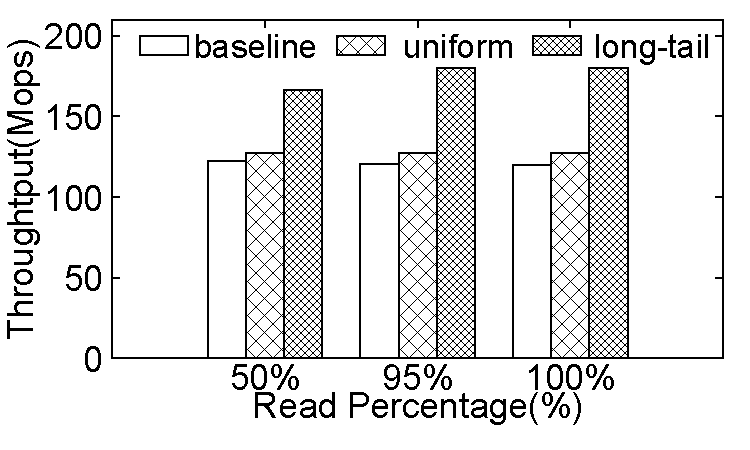
\includegraphics[width=.5\textwidth,page=1]{load_balancer.pdf}}
\caption{负载分派下的 DMA 吞吐量(固定负载分派比例为 0.5)。}
\label{kvdirect:fig:cache-tput}

\end{figure}

\subsubsection{DRAM 负载分配器}
\label{kvdirect:sec:dram-eval}

图 \ref {kvdirect:fig:cache-tput} 显示了仅在使用PCIe的基线上DRAM负载调度的吞吐量改进。
在统一工作负载下,DRAM的缓存效果可以忽略不计,因为它的大小仅为主机键值存储内存的6%。
在长尾工作负载下,大约30%的内存访问由DRAM缓存提供。 总的来说,95%和100%GET的内存访问吞吐量实现了180 Mops的时钟频率限制。
但是,如果简单地将DRAM用作高速缓存,则吞吐量将受到不利影响,因为DRAM吞吐量低于PCIe吞吐量。

\subsubsection{向量操作译码器}
\label{kvdirect:network-eval}

\begin{table}[]
\centering
\scalebox{0.8}{
\begin{tabular}{|l|r|r|r|r|r|}
\hline
向量大小 (字节)              & 64    & 128   & 256   & 512   & 1024  \\ \hline
向量更新(有返回)    & 11.52 & 11.52 & 11.52 & 11.52 & 11.52 \\ \hline
向量更新(无返回) & 4.37  & 4.53  & 4.62  & 4.66  & 4.68  \\ \hline
每个元素一个键         & 2.09  & 2.09  & 2.09  & 2.09  & 2.09  \\ \hline
取回客户端处理             & 0.03  & 0.06  & 0.12  & 0.24  & 0.46  \\ \hline
\end{tabular}
}
\caption{向量操作的吞吐量 (GB/s)。}
\label{kvdirect:tab:vec_throughput}

\end{table}

为了评估键值-Direct中矢量操作的效率,
表 \ref {kvdirect:tab:vec_throughput}将原子矢量增量的吞吐量与两种替代方法进行比较:
(1)如果每个元素都存储为唯一键,则瓶颈是传输键值操作的网络。
(2)如果向量存储为大的不透明值,则向客户端检索向量也会使网络瘫痪。
此外,表 \ref {kvdirect:tab:vec_throughput} 中的两个备选方案不能确保向量内的一致性。 添加同步会产生进一步的开销。

\begin{figure}[t]
\centering
\subfloat[吞吐量。\label{kvdirect:fig:network-batching-bw}]
{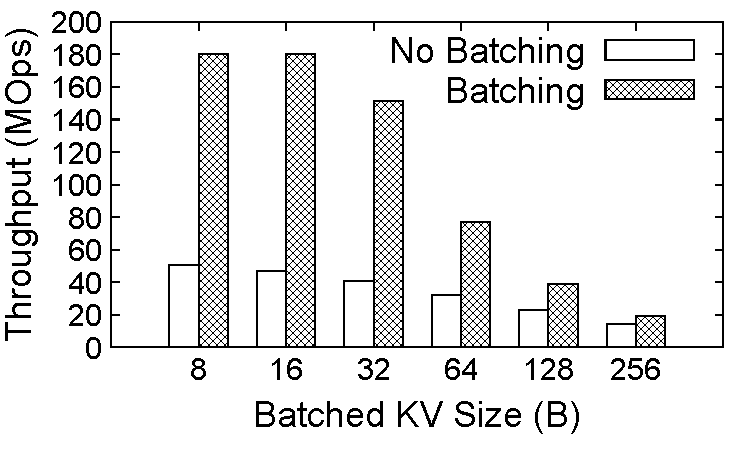
\includegraphics[width=.5\textwidth,page=1]{net_batching_bw.pdf}}
\subfloat[延迟。\label{kvdirect:fig:network-batching-bw}]
{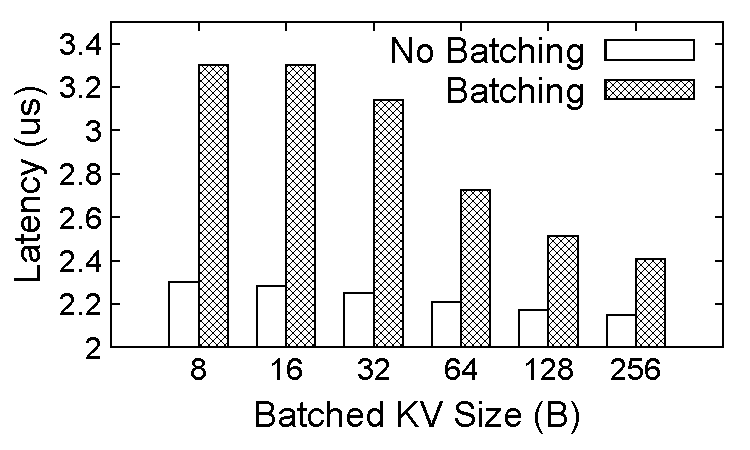
\includegraphics[width=.5\textwidth,page=1]{net_batching_lat.pdf}}
\caption{网络批量化的效率。}
\label{kvdirect:fig:eval-network-batching}

\end{figure}

键值-Direct客户端在网络数据包中打包键值操作,以减轻数据包报头开销。
图 \ref {kvdirect:fig:eval-network-batching} 表明,网络批处理可将网络吞吐量提高4倍,同时保持网络延迟低于3.5~ $ mu $ s。

\egg{
\subsubsection{Congestion Avoidance}
\label{kvdirect:congestion-avoidance}

We evaluate the efficiency of congestion avoidance using the 键值 size distribution of the USR pool in Facebook memcached workload~\cite{atikoglu2012workload}.
As shown in Figure~\ref{kvdirect:fig:congestion-avoidance}, without congestion avoidance, about 70\% 键值 operations complete with close to one PCIe RTT latency, while remaining 30\% operations have inflated completion times due to explicit and implicit queuing in the 键值 processor.
With congestion avoidance, the rate for the programmable NIC to accept 键值 operations from clients is dynamically adjusted, therefore $>$~90\% 键值 operations complete with close to one PCIe RTT latency.
The remaining few percent of operations have intrinsic higher processing delay due to their larger 键值 sizes.
}

\subsection{系统基准测试}
\label{kvdirect:sec:system-benchmark}

\subsubsection{方法}

在每个基准测试之前,我们根据键值大小,访问模式和目标内存利用率来调整哈希索引比率,内联阈值和负载分派比率。
然后我们生成具有给定大小的随机键值对。
给定内联键值大小的密钥大小与键值-Direct的性能无关,因为在处理期间将密钥填充到最长的内联键值大小。
为了测试内联案例,我们使用键值大小作为插槽大小的倍数(当大小为$ \leq $ 50时,即10个插槽)。为了测试非内联的情况,我们使用的键值大小是2减2字节的幂(对于元数据)。
作为准备的最后一步,我们发出PUT操作以将键值对插入空闲键值存储,直到50%内存利用率。
其他内存利用率下的性能可以从图 \ref {kvdirect:fig:mem-access-tput}中获得。

在基准测试期间,我们在同一个ToR中使用基于FPGA的数据包生成器 \cite {li2016clicknp}来生成批量键值操作,将它们发送到键值服务器,接收完成并测量可持续的吞吐量和延迟。
分组生成器的处理延迟通过直接环回预先校准,并从延迟测量中移除。
误差线表示$ 5^{th} $和$ 95^{th} $百分位数。

\subsubsection{吞吐量}

\begin{sidewaystable}[h]
\centering
\begin{tabular}{|l|l|l|r|r|r|r|r|r|r|}
\toprule
键值存储  & 注释 & 性能瓶颈 & \multicolumn{2}{c|}{吞吐量 (Mops)} & \multicolumn{2}{c|}{功耗效率 (Kops/W)} & \multicolumn{2}{c|}{平均延迟 ($\mu$s)} \\
\cline{4-9}
 & & & GET & PUT & GET & PUT & GET & PUT \\
\midrule
Memcached~\cite{fitzpatrick2004distributed} & Traditional & Core synchronization & 1.5 & 1.5 & \approx5 & \approx5 & \approx50 & \approx50 \\
MemC3~\cite{fan2013memc3} & Traditional & OS network stack & 4.3 & 4.3 & \approx14 & \approx14 & \approx50 & \approx50 \\
RAMCloud~\cite{ousterhout2015ramcloud} & Kernel bypass & Dispatch thread & 6 & 1 & \approx20 & \approx3.3 & 5 & 14 \\
MICA~\cite{lim2014mica} & Kernel bypass, 24 cores, 12 NIC ports & CPU 键值 processing & 137 & 135 & 342 & 337 & 81 & 81 \\
FaRM~\cite{dragojevic2014farm} & One-sided RDMA for GET & RDMA NIC & 6 & 3 & \approx30 (261) & \approx15 & 4.5 & \approx10 \\
DrTM-键值~\cite{wei2015fast} & One-sided RDMA and HTM & RDMA NIC & 115.2 & 14.3 & \approx500 (3972) & \approx60 & 3.4 & 6.3 \\
HERD'16~\cite{kalia2016design} & Two-sided RDMA, 12 cores & PCIe & 98.3 & \approx60 & \approx490 & \approx300 & 5 & 5 \\
Xilinx'13~\cite{blott13hotcloud} & FPGA (with host) & Network & 13 & 13 & 106 & 106 & 3.5 & 4.5 \\
Mega-键值~\cite{zhang2015mega} & GPU (4~GiB on-board RAM) & GPU 键值 processing & 166 & 80 & \approx330 & \approx160 & 280 & 280 \\
\midrule
\textbf{键值-Direct (1 NIC)} & Programmable NIC, two Gen3 x8 & PCIe \& DRAM & 180 & 114 & 1487 (5454) & 942 (3454) & 4.3 & 5.4 \\
\textbf{键值-Direct (10 NICs)} & Programmable NIC, one Gen3 x8 each & PCIe \& DRAM & 1220 & 610 & 3417 (4518) & 1708 (2259) & 4.3 & 5.4 \\
\bottomrule
\end{tabular}
\caption{键值-Direct 与其他键值存储系统在长尾(倾斜  Zipf)负载和 10 字节小键下的比较。对于相关工作未报告的性能数字,我们使用相似的硬件来模拟这些系统,并报告我们粗略的测量结果。对于 CPU 绕过的系统,括号内的数字报告峰值负载和空闲情况下的功耗差异。}
\label{kvdirect:tab:kvs-compare}

\end{sidewaystable}

\begin{figure}[t]
\centering
\subfloat[均匀分布。\label{kvdirect:fig:ycsb-tput-uniform}]
{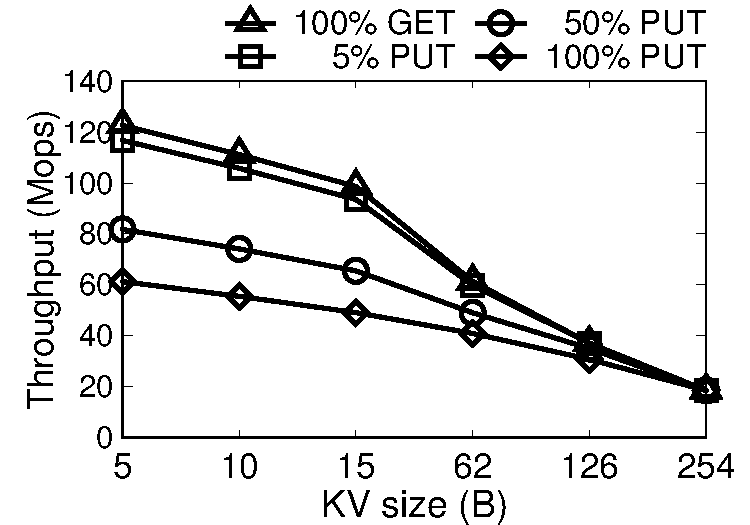
\includegraphics[width=.5\textwidth,page=1]{ycsb-tput-uniform.pdf}}
\subfloat[长尾分布。\label{kvdirect:fig:ycsb-tput-longtail}]
{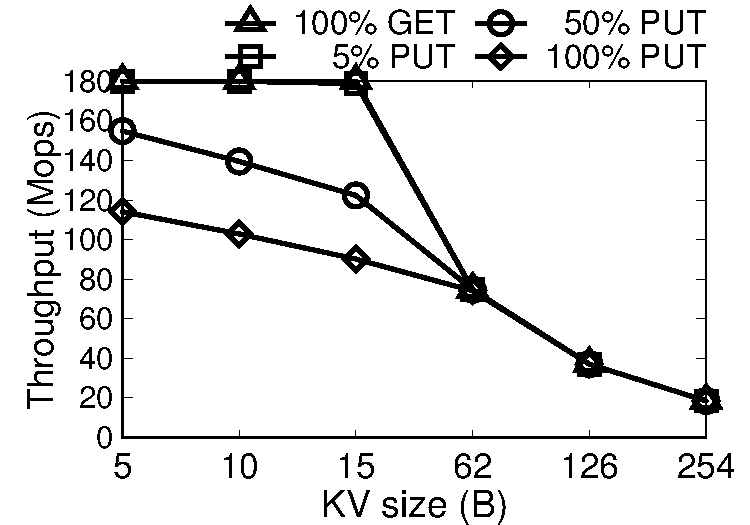
\includegraphics[width=.5\textwidth,page=1]{ycsb-tput-longtail.pdf}}
\caption{键值-Direct 在 YCSB 负载下的吞吐量。}
\label{kvdirect:fig:ycsb-tput}

\end{figure}

图 \ref {kvdirect:fig:ycsb-tput} 显示了YCSB均匀和长尾(偏斜Zipf)工作负载下键值-Direct的吞吐量。
三个因素可能是键值-Direct的瓶颈:时钟频率,网络和PCIe / DRAM。
对于在散列索引中内联的5B至15B 键值,大多数GET需要一个PCIe / DRAM访问,而PUT需要两个PCIe / DRAM访问。
这种小型键值在许多系统中很普遍。在PageRank中,边的键值大小为8B。在稀疏逻辑回归中,键值大小通常为8B-16B。对于分布式系统中的顺控程序和锁定,键值大小为8B。

在相同的内存利用率下,由于哈希冲突的概率较高,较大的内联键值具有较低的吞吐量。
62B和更大的键值没有内联,因此它们需要额外的内存访问。
长尾工作负载比统一工作负载具有更高的吞吐量,并且能够在读密集工作负载下达到180~Mops的时钟频率范围,或达到$ \geq $ 62B 键值大小的网络吞吐量。
在长尾工作负载下,无序执行引擎在最流行的密钥上合并到大约15%的操作,并且板载DRAM在60%负载分配比率下具有大约60%的高速缓存命中率,这可以统一导致高达2倍的吞吐量作为统一的工作量。
如表 \ref {kvdirect:tab:kvs-compare} 所示,键值-Direct NIC的吞吐量与具有数十个CPU核心的最先进的键值存储服务器相当。

\subsubsection{能耗效率}

插入键值-Direct NIC可为空闲服务器增加10.6 W的功率。
当键值-Direct服务器处于峰值吞吐量时,系统功率为121.4瓦(在墙上测量)。
与表 \ref {kvdirect:tab:kvs-compare} 中最先进的键值存储系统相比,键值-Direct的功率效率是其他系统的3倍,是第一个达到100万的通用键值存储系统 商用服务器上每瓦特的键值操作。

当拔出键值-Direct网卡时,空闲服务器的功耗为87.0瓦,因此可编程网卡,PCIe,主机内存和CPU上的守护进程的总功耗仅为34瓦。
测量的功率差异是合理的,因为CPU几乎处于空闲状态,服务器可以在键值-Direct运行时运行其他工作负载(我们对单侧RDMA使用相同的标准,如表 \ref {kvdirect:tab:kvs} 的括号中所示)。
在这方面,键值-Direct的功率效率是基于CPU的系统的10倍。

\subsubsection{延迟}
\begin{figure}[t]
\centering
\subfloat[With batching.\label{kvdirect:fig:ycsb-lat-batch}]
{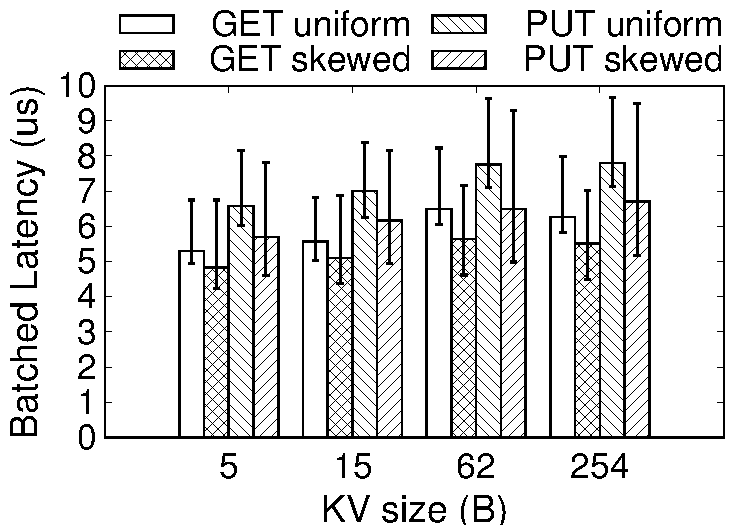
\includegraphics[width=.5\textwidth,page=1]{lat-batch.pdf}}
\subfloat[Without batching.\label{kvdirect:fig:ycsb-lat-nobatch}]
{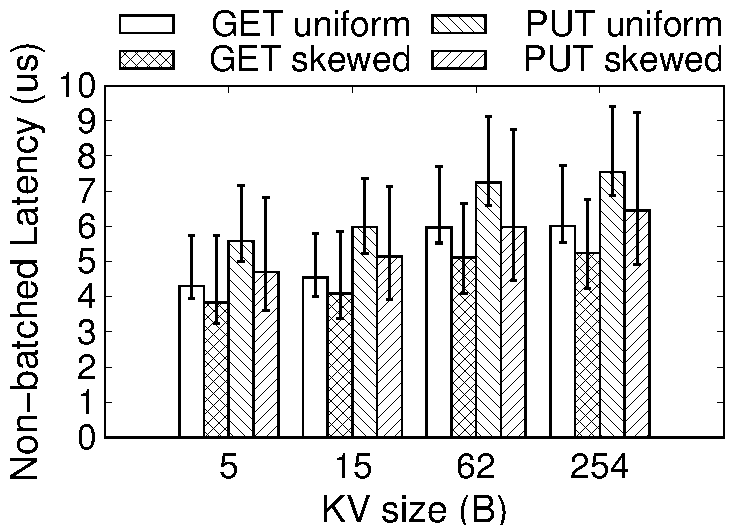
\includegraphics[width=.5\textwidth,page=1]{lat-nonbatch.pdf}}
\caption{在YCSB工作负载的峰值吞吐量下键值-Direct的延迟。}
\label{kvdirect:fig:ycsb-lat}

\end{figure}

图 \ref {kvdirect:fig:ycsb-lat} 显示了YCSB工作负载峰值吞吐量下键值-Direct的延迟。
在没有网络批处理的情况下,尾部延迟范围为3至9 $\mu$s,具体取决于键值大小,操作类型和密钥分配。
由于额外的内存访问,PUT具有比GET更高的延迟。
由于更有可能在板载DRAM中进行缓存,因此倾斜的工作负载具有比均匀更低的延迟。
由于额外的网络和PCIe传输延迟,较大的键值具有较高的延迟。
网络批处理比非批处理操作增加了不到1~$\mu$s 的延迟,但显着提高了吞吐量,已在图 \ref {kvdirect:fig:eval-network-batching} 中进行了评估。

\subsubsection{对 CPU 性能的影响}

\begin{table}[htbp]
	\centering
		\begin{tabular}{l|l|r|r}
			\toprule
			\multicolumn{2}{r}{键值-Direct status $\rightarrow$} & Idle & Busy \\
			\midrule
			\multirow{4}{*}{\specialcell{Random\\Latency}} & CPU0-0 & 82.2 ns & 83.5 ns \\
            					  & CPU0-1 & 129.3 ns & 129.9 ns \\
                                  & CPU1-0 & 122.3 ns & 122.2 ns \\
                                  & CPU1-1 & 84.2 ns & 84.3 ns \\
			\midrule
            \multirow{4}{*}{\specialcell{Sequential\\Throughput}} & \textbf{CPU0-0} & \textbf{60.3 GB/s} & \textbf{55.8 GB/s} \\
            					  & CPU0-1 & 25.7 GB/s & 25.6 GB/s \\
                                  & CPU1-0 & 25.5 GB/s & 25.9 GB/s \\
                                  & CPU1-1 & 60.2 GB/s & 60.3 GB/s \\
			\midrule
			\multirow{4}{*}{\specialcell{Random\\Throughput}} & 32B read & 10.53 GB/s & 10.46 GB/s \\
            						& 64B read & 14.41 GB/s & 14.42 GB/s \\
                                    & 32B write & 9.01 GB/s & 9.04 GB/s \\
                                    & 64B write & 12.96 GB/s & 12.94 GB/s \\
			\bottomrule
		\end{tabular}
    	\caption{当键值-Direct达到峰值吞吐量时,对CPU内存访问性能的影响。 使用英特尔性能计数器监视器V2.11测量。}
        \label{kvdirect:tab:cpu-impact}
        
\end{table}

键值-Direct旨在绕过服务器CPU,仅使用一部分主机内存用于键值存储。 因此,CPU仍然可以运行其他应用程序。
当单个NIC 键值-Direct处于峰值负载时,我们的测量结果对服务器上的其他工作负载的影响最小。
表 \ref {kvdirect:tab:cpu-impact} 量化了键值-Direct峰值吞吐量的影响。
除了CPU 0的顺序吞吐量以访问其自己的NUMA内存(以粗体标记的行)之外,CPU内存访问的延迟和吞吐量大多不受影响。
这是因为8个主机存储器通道可以提供比所有CPU核心消耗的更高的随机访问吞吐量,而CPU确实可以强调DRAM通道的顺序吞吐量。
当键值大小的分布相对稳定时,主机守护程序进程的影响是最小的,因为仅当不同板大小的可用槽的数量不平衡时才调用垃圾收集器。
